%!TEX root = ../master.tex
\chapter{Design}\label{ch:design}
bla bla bla intro to chapter here.

\section{An interactive board for Terra Mystica}
This project aims to create an interactive board for Terra Mystica, using computer vision to detect hand contact on the board via a camera below its surface. With the hand contact, the user should be able to change the colour of the hexagon-shaped tiles in the game. The idea is that the board itself is a projection from below, and the board should change according to inputs on board's surface.

The interactive board will eliminate the need for terrain game pieces, since it will manage terraforming digitally for the player. It may also assist the players in remembering the Power mechanic, as well as streamline other elements of the game.

A possible expansion of the project would be detection of game pieces, which can be used to measure amount of power to be offered after game piece placement.

\section{Lo-fi test}
\begin{figure}
\centering
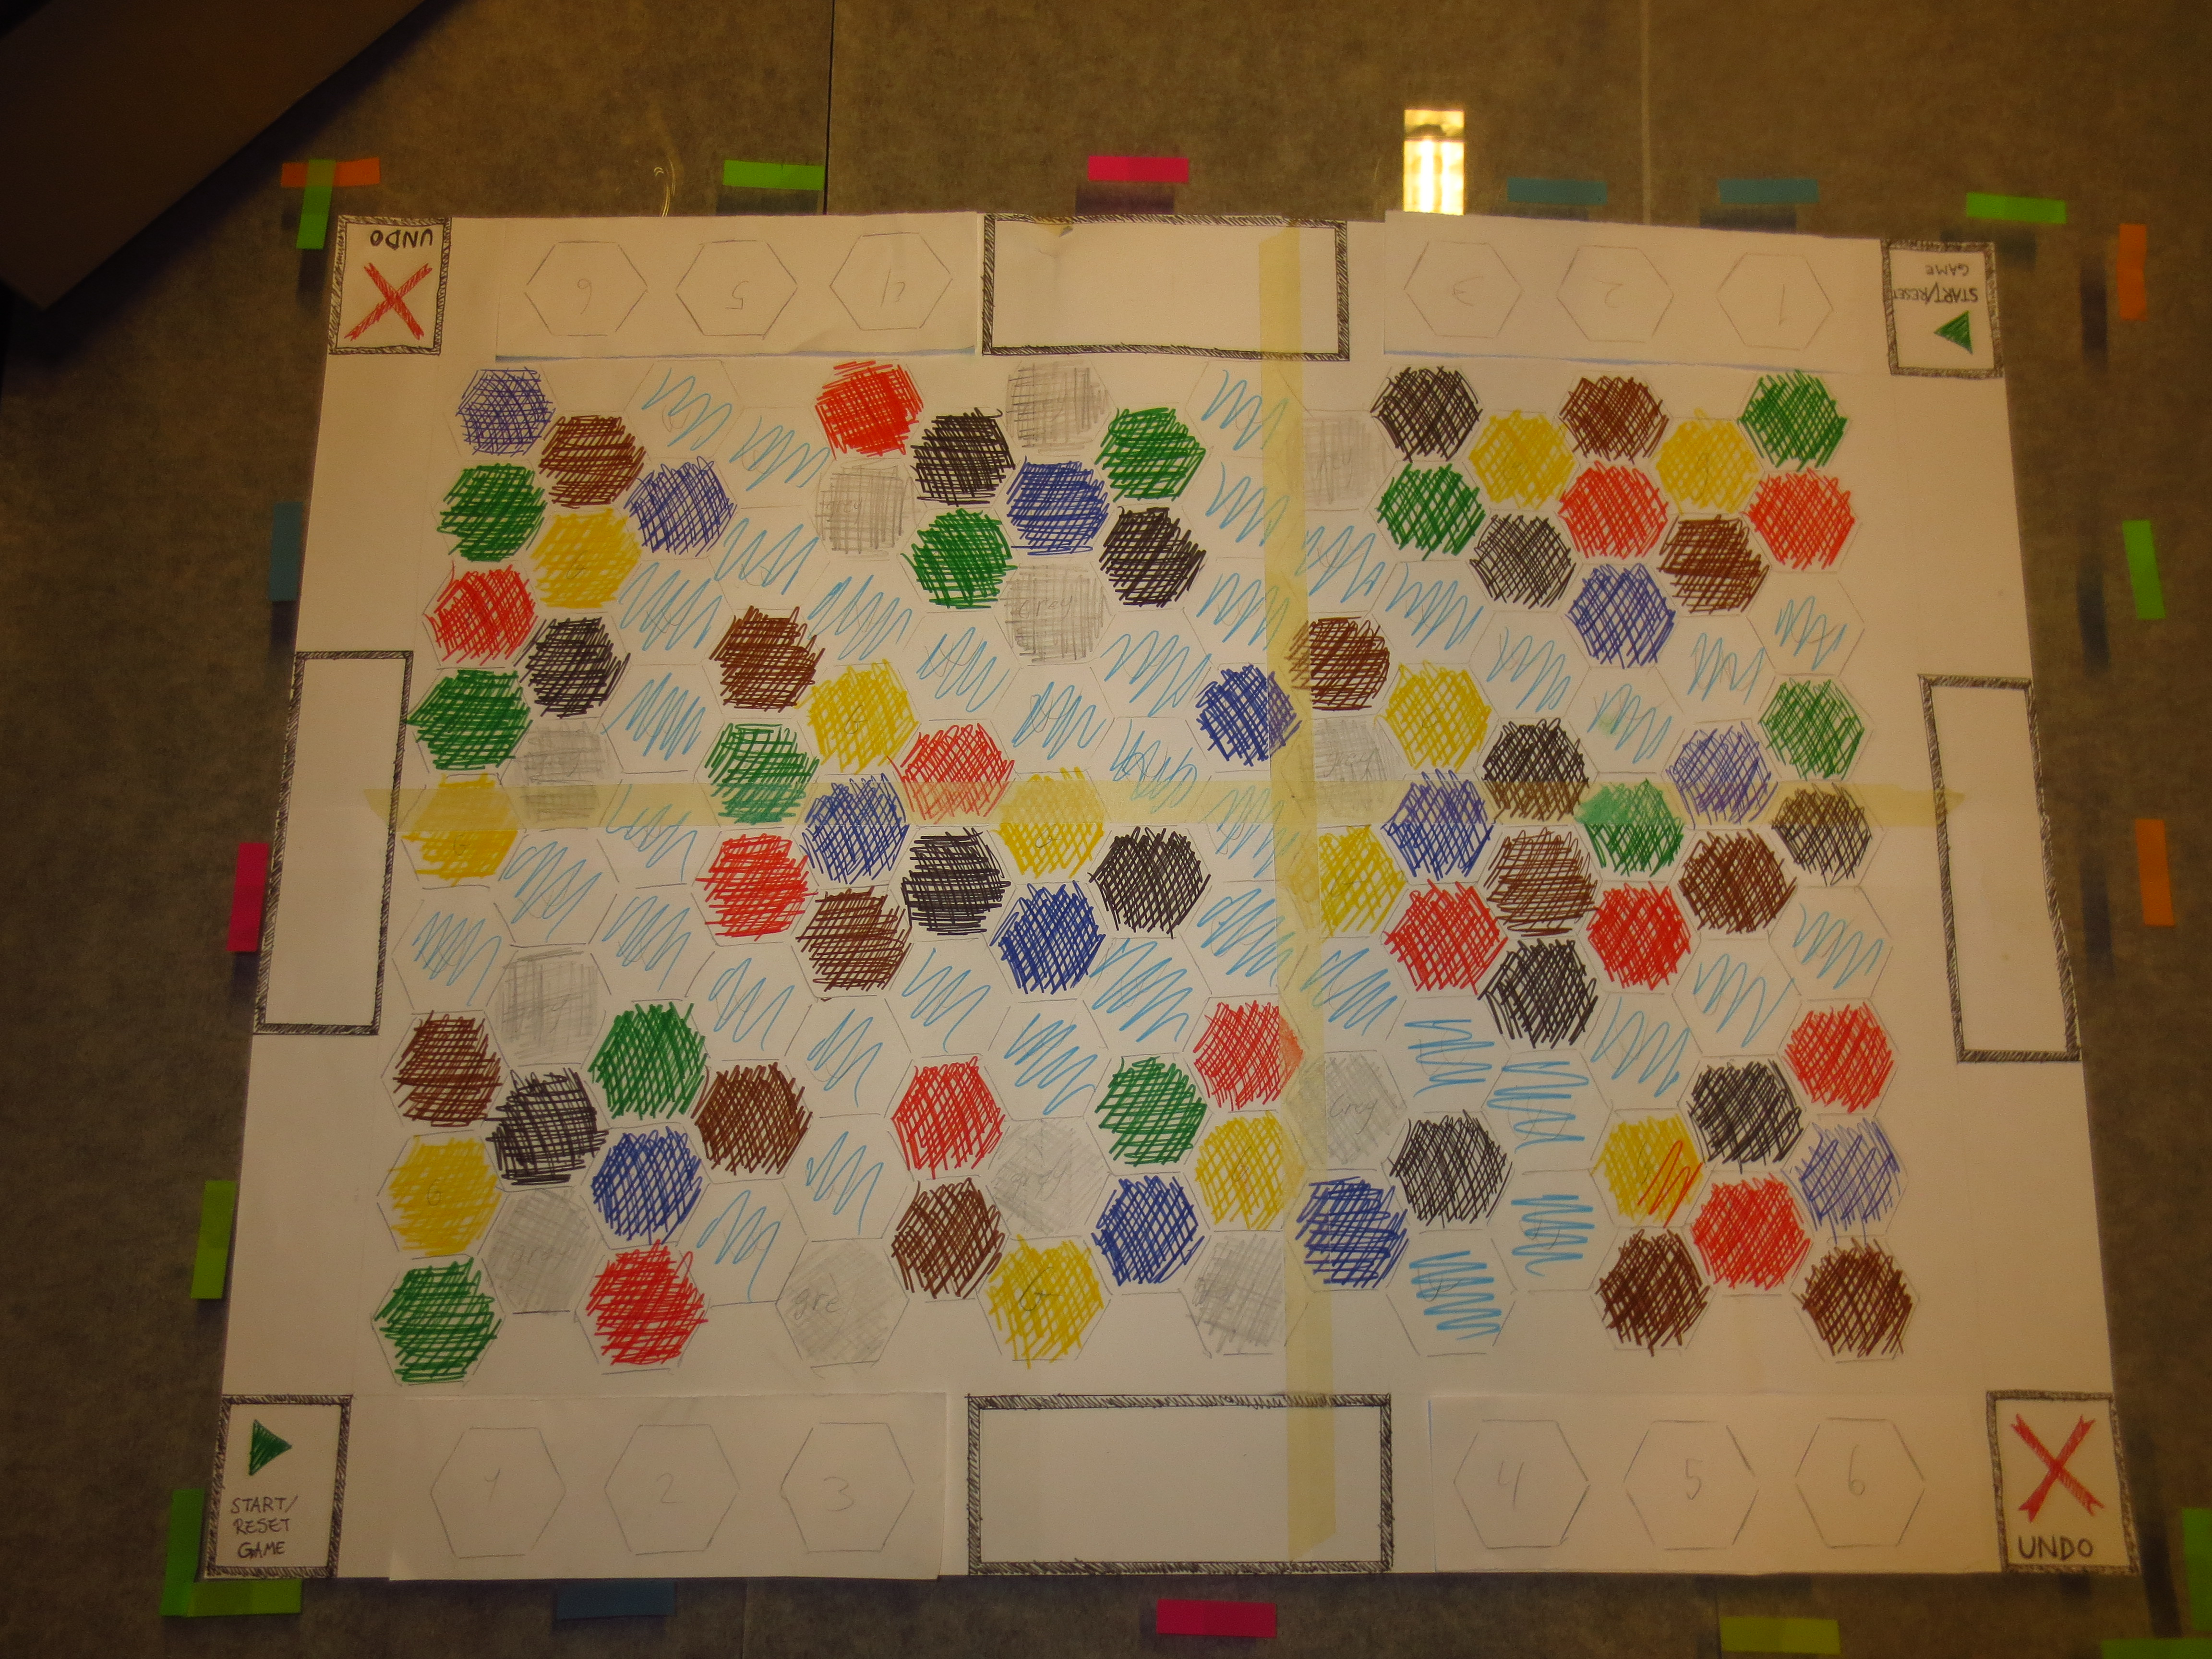
\includegraphics[width=0.9\textwidth]{IMG_0001}
\caption{The Lo-Fi board}
\end{figure}

After defining the initial design a lo-fi test was conducted to test whether the areas of interest were large enough, the defined gestures were easy to perform and if the increased size had any effect on the gameplay. We also wanted a first outside opinion of the game without the terraforming pieces. 

For the lo-fi we had three participants: Nadia, Catja and Sebastian. \todo{Probably need their entire names here} 
They were all familiar with the game Terra Mystica so they did not need to learn the game first. They only played two rounds since one of the key points of the test was to learn if the gestures and the areas were good. 

They all had a little bit of trouble remembering to do the terraforming gesture in the beginning, but they were all pretty sure that with a little more playing it would come naturally/it would be fine. They also mentioned that it might be easier to remember to do the start of turn gesture if the non touch areas of the board lit up in their respective colours. 

They generally liked the bigger board since this made the hexes and other touch areas bigger, but they did also mention that for short people it might be a problem to reach the other end of the board. 

The mix of tangible and “digital” elements was confusing for the participants. They felt that it would make more sense to have the buildings digital but on the other hand they also felt that that would remove the tangibility that they like about the game. They mentioned that it might help to indicate where or when you want to build/upgrade since only doing a gesture whenever you need to terraform seems a bit odd. 

The personal player input area could be utilised better. Maybe it could indicate income or victory points or just indicate whenever it is your turn. 

The conclusions of the lo-fi test are that they gestures are easy to do and the areas of interest are large enough. The increased size of the board did make it harder for smaller players. The next step is then to discern if the programme will be able to recognise the gestures. 

\subsection{Procedure}
First participants were chosen from those who already knew the game.
Then they were introduced to the Lo-Fi board, by the primary interviewer who also acted as the "programme", about how the gestures worked and where they worked. They then played two rounds of the game, with some functions removed since they had no effect when only playing two rounds. During the game they commented out loud, which was noted down by the secondary interviewer who also noted down their reactions and behaviour. 
After the game they were asked some questions in a loosely structured group interview. 
The whole test was filmed.

\subsection{title placeholder} \todo{this title should be changed. the section will be about the gui design and needs/nice to haves}
hahaha

\begin{figure}
\centering
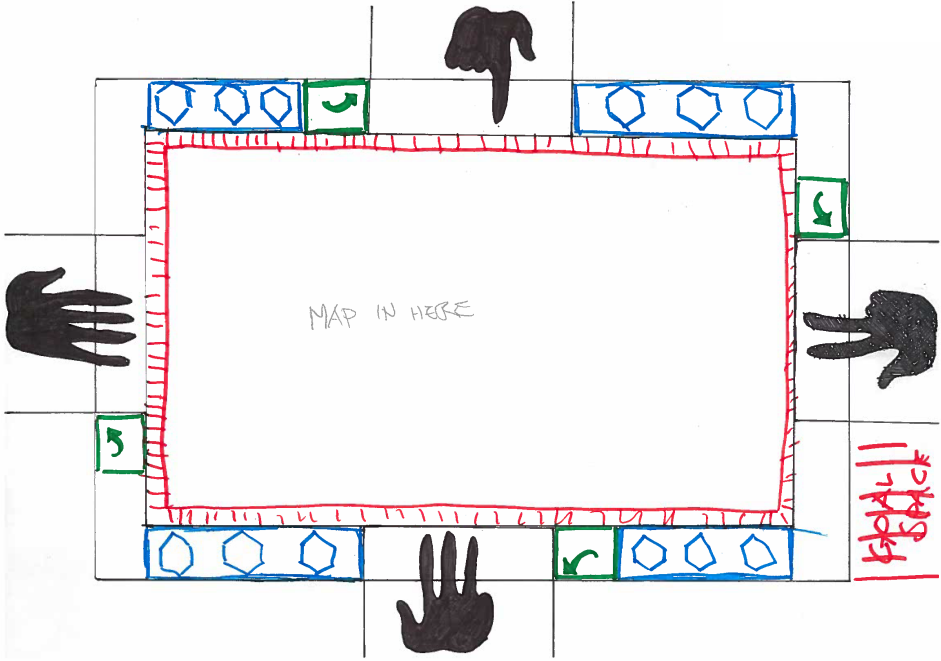
\includegraphics[width=0.9\textwidth]{sketchGUI}
\caption{Sketch illustrating the interface}
\end{figure}

\section{Requirement specifications} \todo {Not sure if this is the right place to have this}
The following is the specifications of the usability- and software-based requirements needed in order to to design, build and program the interactive board for Terra Mystica.

\begin{itemize}
\item Must be able to read whether one, two, three, or four fingers have been placed on one of the player selection areas.
	\begin{itemize}
	\item Each of these four players must have a corresponding terrain type, represented by a colour.
	\item This must be successful 90\% of the time (note - type of tile placement depends of player selected, which makes its success significant).
	\end{itemize}
\item Once the player is selected, the program must be able to detect when a tile is selected for terraforming - that is, when a player places three fingers on the hexagon in question. This tile must then change to the terrain type, that is, the colour, of the last player who was selected.
	\begin{itemize}
	\item This must be successful 75\% of the time.
	\end{itemize}
\item In case of misplacement of terraforming, the program must be able to detect the use of an undo-button, which should be done with the same input as with the terraforming, but in a different area of interest.
	\begin{itemize}
	\item This must be successful 50\% of the time, since its function is not the most crucial for the program’s presupposed run of a game.
	\item The undo-buttons area of interest needs to be secluded from the other areas of interest, so it can not accidentally be interacted with. 
	\end{itemize}
\item In the game, there are actions which all players can take, but they can only be taken once per round. In the analogue game, a token is placed on the icon for the action when this happens. For the minimum implementation, this does not need to be managed digitally. However, there should be spaces on the board showing the different actions, on which the players can place tokens in order to remember which actions are already taken. There are six of these actions in total. All of these actions should be represented on the board twice; once on each side of the board, so that they are reachable by all players. This is shown in figure 5.2, where the actions are the blue areas. 
	\begin{itemize}
	\item A further implementation which is nice to have is to make the actions managed digitally. When an action is used, the player must select the action they wish to use by placing three fingers on it, in the same manner as when terraforming. Doing this should toggle the action on and off. When the action is turned off, a cross should appear on the action area, showing the players that the action can now not be used.
	\end{itemize}
\item The digital board should have a point counter. That is, a border around the board consisting of 100 tiles numbered 1-100. The red border on figure 5.2 shows its placement. This border should not be managed digitally, but the players should be able to move a coloured token representing themselves from tile to tile, visualising how many points they have. The program should ignore the tokens placed on this border, by for example having it outside areas of interest. 
\end{itemize}